\documentclass{article}
\usepackage[utf8]{inputenc}
\usepackage{amsmath}
\usepackage{amsfonts}
\usepackage{graphicx}

\title{Stochastic Processes}
\author{Grant Smyth }
\date{Spring 2022}

\begin{document}

\maketitle

\section{Introduction}
We are just going to show a few things about stochastic integration and differentiation.

$$X_t = x : \Omega \rightarrow \mathbb{R}^+ \rightarrow  \mathbb{R} = x :  \left(\Omega  , \mathbb{R}^+\right)\rightarrow  \mathbb{R}$$ 

And we have that

$$x(\varsigma_1) = f_1(t)$$
$$x(\varsigma_2) = f_2(t)$$
$$x(\varsigma) = f_\varsigma(t)$$

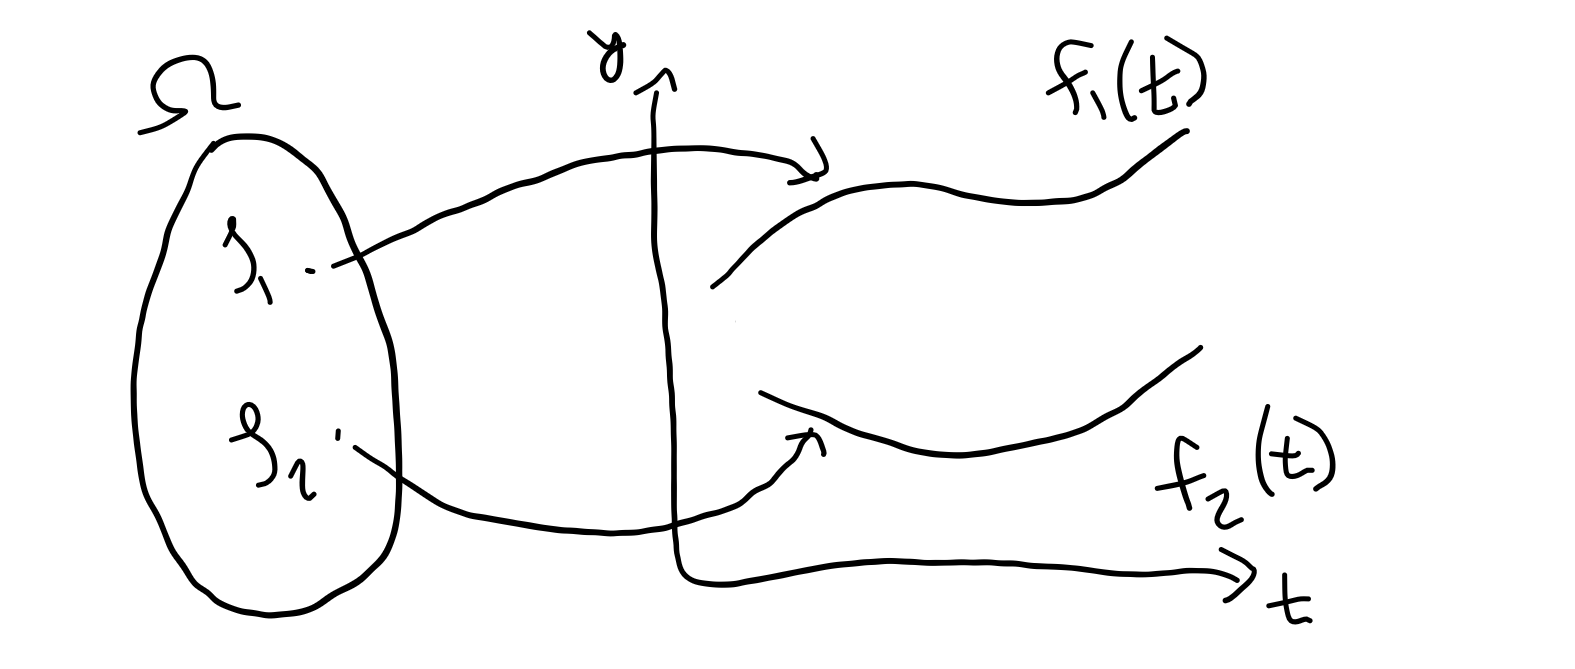
\includegraphics[width=\textwidth]{stochastic_ image.png}

\newpage

\subsection{Differentiation}
We have that:

$$X_t' = \frac{\partial x}{\partial t}\left(\varsigma, t\right)=g\left(\varsigma, t\right) = \frac{x\left(\varsigma, t + h\right) - x\left(\varsigma, t\right)}{h} = \frac{f_\varsigma\left(t + h\right) - f_\varsigma\left(t\right)}{h} = \frac{df_\varsigma}{dt}$$

Which means that $X_t'$ is just the probability weighted derivatives of the trajectories.

Side note that this does not work in Brownian Motion because the individual trajectories in Brownian Motion are not differentiable (anywhere).  I think we might be able to do it with some form of a weak derivative, though, just not the regular one.

\subsection{Integration}
We have that:
$$\int X_t = h\left(\varsigma,t\right)= \int_{s = 0}^{s = t} X_s ds = \int_{s = 0}^{s = t} x\left(\varsigma,s\right) ds = \int_{s = 0}^{s = t} f_\varsigma\left(s\right) ds $$

Which means that $\int X_t$ is just the probability weighted integrals of the trajectories.

I think we can do this with Brownian Motion because even though Brownian Motion trajectories are not (in the normal sense) differentiable, they are integrable.

\end{document}
